\documentclass{standalone}
\usepackage{tikz}
\usetikzlibrary{arrows.meta}

\begin{document}
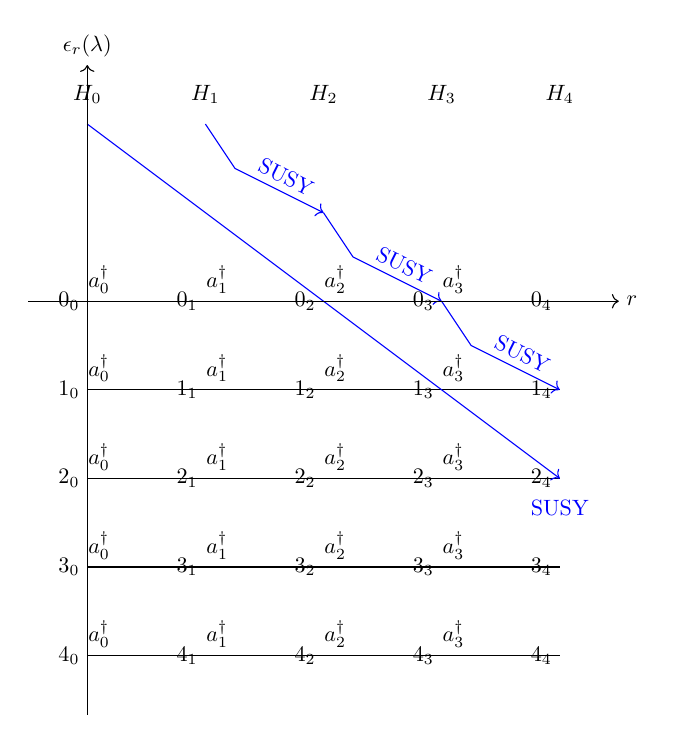
\begin{tikzpicture}[scale=0.75, every node/.style={scale=0.8}]
    % Draw the states
    \foreach \i in {0,...,4} {
        \draw (0, -\i*1.5) node[left] {$\ket{\i}_0$};
        \draw (2, -\i*1.5) node[left] {$\ket{\i}_1$};
        \draw (4, -\i*1.5) node[left] {$\ket{\i}_2$};
        \draw (6, -\i*1.5) node[left] {$\ket{\i}_3$};
        \draw (8, -\i*1.5) node[left] {$\ket{\i}_4$};
    }

    % Draw the Hamiltonian labels
    \foreach \i in {0,...,4} {
        \draw (0, -\i*1.5) -- node[above, pos=0.1] {$a_0^\dagger$} (2, -\i*1.5);
        \draw (2, -\i*1.5) -- node[above, pos=0.1] {$a_1^\dagger$} (4, -\i*1.5);
        \draw (4, -\i*1.5) -- node[above, pos=0.1] {$a_2^\dagger$} (6, -\i*1.5);
        \draw (6, -\i*1.5) -- node[above, pos=0.1] {$a_3^\dagger$} (8, -\i*1.5);
    }

    % Draw the Hamiltonian names
    \node at (0, 3.5) {$H_0$};
    \node at (2, 3.5) {$H_1$};
    \node at (4, 3.5) {$H_2$};
    \node at (6, 3.5) {$H_3$};
    \node at (8, 3.5) {$H_4$};

    % Draw the SUSY arrows
    \draw[->, blue] (2, 3) -- (2.5, 2.25) -- node[above, sloped] {SUSY} (4, 1.5);
    \draw[->, blue] (4, 1.5) -- (4.5, 0.75) -- node[above, sloped] {SUSY} (6, 0);
    \draw[->, blue] (6, 0) -- (6.5, -0.75) -- node[above, sloped] {SUSY} (8, -1.5);
    \draw[->, blue] (0, 3) -- (8, -3) node[right, black] {};
    \node[blue] at (8, -3.5) {SUSY};

    % Draw the axis labels
    \draw[->] (-1,0) -- (9,0) node[right] {$r$};
    \draw[->] (0,-7) -- (0,4) node[above] {$\epsilon_r(\lambda)$};
\end{tikzpicture}
\end{document}